\section{Experiments}

\subsection{General Experiment Setup}
We consider 63 condition predicates and 20 action predicates in the predicate set $\PredicateSet$.
All predicates are categorized into four types: (1) safety-related (e.g., will the plan result in obstacle collision?) (2) comfort-related (e.g., is the acceleration in a reasonable range?); (3) efficiency-related (e.g., is the car is in a slow lane?); (4) environment-related (e.g., is the curvature of the current lane too high?).
Implementing the predicate set $\PredicateSet$ involves LLM-aided design \cite{Chen2022CodeTCG}, but the final predicates were manually checked to ensure correctness and sensibility.

We used all the NuPlan demonstrations in Singapore, Pittsburgh, and Boston, and part of the demonstrations in Las Vegas, to train the logic structure. The scenarios are grouped into 9 types (the first column in Table \ref{tab: closed-loop-planning-performance}). The dataset is split into 90\% training and 10\% validation. The validation set is used for hyperparameter tuning and early stopping. Following PDM \cite{Dauner2023CORL}, we use the log replay to obtain the 4-second future trajectories of other agents in both training and evaluation.

We trained an ensemble $\LogicStucture_{\mathit{ensemble}}$ with 10 different $\LogicStucture$. Each $\LogicStucture$ has 2 layers of the Temporal layer. The single class regularization parameters $\alpha$ and $\beta$ are set to $10^{-5}$ and $10^{-3}$, respectively. The learning rate is set to $10^{-4}$, and optimized with the Adam optimizer. The batch size is set to 32. The training process is stopped when the validation loss does not decrease for 10 epochs. We used 15 trajectory candidates for evaluation in closed-loop simulation.

\subsection{Case Study}
\subsubsection{Logic Rules Discovered}
\label{sec:logic_rules_discovered}

Fig.~\ref{fig:motivation_example} shows three of the rules learned by the grading logic network. Given the motion plan proposed by PDM \cite{Dauner2023CORL}, the grading logic network assigns a score to each plan based on the learned rules. Fig.~\ref{fig:case-study-example} shows why the \textcolor[HTML]{2278B4}{blue}, \textcolor[HTML]{D52928}{red} and \textcolor[HTML]{F98217}{orange} plans receive lower scores. The blue plan receives a low score for going beyond the drivable area (the gray area), which violates the rule $\top \rightarrow \mathbf{G} \mathit{InDrivable}$. The red plan is penalized for exceeding comfort constraints (the blue dashed line) on lateral acceleration, which violates the rule $\mathbf{G} \mathit{SafeTTC} \rightarrow \mathbf{G} \mathit{Comfortable}$. The orange plan receives a lower score for exceeding the speed limit (the red dashed line) when not overtaking another vehicle, which violates the rule $\lnot \mathit{SpeedLimit} \rightarrow \mathbf{F} \mathit{Overtaking}$. These rules are almost always discovered in our experiment. One exception is that the rule $\lnot \mathit{SpeedLimit} \rightarrow \F \mathit{Overtaking}$ could sometimes devolve to  $\mathit{SpeedLimit}$ or $\G \mathit{SpeedLimit}$   in scenarios where overtaking happens rarely (e.g., following other cars). More detailed case studies are provided on our website.

\begin{figure}[h!]
    \centering
    % \vspace{-.3cm}
    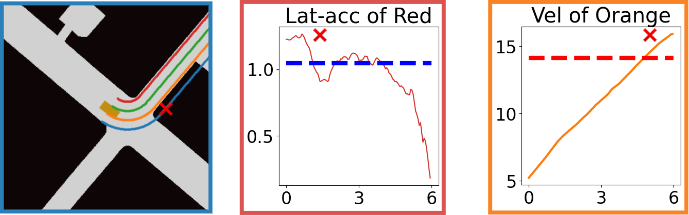
\includegraphics[width=\linewidth]{imgs/case_study.drawio.png}
    % \vspace{-.3cm}
    \caption{
        Case study on discovered rules. While our method evaluates 15 trajectory candidates in practice, we show only 4 representative trajectories here for visual clarity. From left to right, these sub-figures explain why the blue, red, and orange plans received lower scores. The blue plan violates the drivable area rule, the red plan exceeds comfort constraints on lateral acceleration, and the orange plan breaks the speed limit without overtaking context.
    }
    % \vspace{-.3cm}
    \label{fig:case-study-example}
\end{figure}


\subsubsection{Parameter Optimization}

$\mathit{Comfortable}_{\boldsymbol{\theta}}$ is a predicate measure if a motion plan is comfortable, which has parameters $\boldsymbol{\theta} = [\theta_{a_{f}}, \theta_{a_{b}}, \theta_{a_{l}}, \theta_{a_{r}}]$, representing thresholds for acceleration in forward, backward, left, and right directions. It can be defined as:
\begin{align}
    \mathit{Comfortable}_{\boldsymbol{\theta}} := \tanh(\min_{\substack{i \in \{a_{f}, a_{b}, a_{l}, a_{r}\}}} \{\theta_i - i(\tau)\})
\end{align}
\label{eq:comfortable_predicate}
where $i(\tau)$ represents the maximum acceleration in the plan $\tau$ for each respective direction.
Only when all the accelerations are below their thresholds, is the predicate evaluated as positive. The $\tanh$ function is used to ensure the output is in $[-1, 1]$. All threshold parameters in \eqref{eq:comfortable_predicate} are differentiable and can be learned from the training demonstration data.
The learned parameters $\boldsymbol{\theta}$ are shown in Table \ref{tab: parameter-optimization}.

\begin{table}[!htp]\centering
    % \vspace{-0.3cm}
    \caption{Case Study on Learned Parameters of $\mathit{Comfortable}_{\boldsymbol{\theta}}$}\label{tab: parameter-optimization}
    % \vspace{-.3cm}
    \scriptsize
    \begin{tabular}{l|cccc}\toprule
                          & $\theta_{a_{f}}$ & $\theta_{a_{b}}$ & $\theta_{a_{l}}$ & $\theta_{a_{r}}$ \\\midrule
        \textbf{Standard} & 1.23             & 1.13             & 0.98             & 0.98             \\
        \textbf{Learned}  & 1.1  $\pm$ 0.21  & 1.045 $\pm$ 0.12 & 0.9 $\pm$ 0.11   & 0.95 $\pm$ 0.51  \\
        \bottomrule
    \end{tabular}
    \begin{tablenotes}
        \item The learned parameters are shown in the format of mean $\pm$ standard deviation computed from 5 independent runs.
    \end{tablenotes}
    % \vspace{-.3cm}
\end{table}

The \textbf{Standard} parameters of comfortable acceleration are provided in \cite{deWinkel2023Standards} from a user study.
We observe the \textbf{Learned} parameters are close to \textbf{Standard}. In practice, it is noticeable that the acceleration thresholds are hard to estimate. However, the learned parameters are comparable to the standard values by learning from data, which indicates the proposed method can learn the parameters characterizing the demonstration data well. The notable standard deviations in Table~\ref{tab: parameter-optimization} reflect inherent variations in driving behavior, from right turns showing higher variation than left turns, to forward acceleration varying more than deceleration. These variations persist despite analyzing over 100 hours of driving data, suggesting they stem from inherent differences in driving environments (e.g., Boston's narrow streets versus Las Vegas's wide boulevards) rather than insufficient data. Potentially, better scenario-based classification could address these variations, but we leave this for future work.

\subsection{Evaluation in Closed-loop Planning}

The learned rules are evaluated in a closed-loop planning system using NuPlan under two settings: Closed-Loop Score Non-Reactive (CLS-NR), where other agents follow recorded trajectories, and Closed-Loop Score Reactive (CLS-R), where agents are controlled by an Intelligent Driver Model (IDM) policy. Performance is measured using normalized scores (0-1) across safety (collision avoidance, following distances), rule compliance (lane keeping, speed limits), progress along the route, and comfort (acceleration, jerk), assessing the rules' ability to balance driving requirements in both predictable and interactive scenarios. The results are shown in Table \ref{tab: closed-loop-planning-performance}. Here, we compare our learned Scoring Logic Network (SLN) with the Expert Rules (ER) in PDM \cite{Dauner2023CORL} and the Neural Critic (NC) \cite{jiang2022efficient}. The last two rows show the overall performance on ``All'' the scenarios and the Val14 split originally used for evaluating the ER \cite{Dauner2023CORL}.

\begin{table}[!htp]\centering
    % \vspace{-0.3cm}
    \caption{Closed-Loop Planning Performance}
    \label{tab: closed-loop-planning-performance}
    % \vspace{-.3cm}
    \scriptsize
    \begin{tabular}{l@{\hspace{0.8em}}|c@{\hspace{0.8em}}c@{\hspace{0.8em}}c@{\hspace{0.8em}}|c@{\hspace{0.8em}}c@{\hspace{0.8em}}c@{\hspace{0.8em}}|c@{\hspace{0.8em}}c@{\hspace{0.8em}}c}\toprule
                    & \multicolumn{3}{c}{Rule Complexity} & \multicolumn{3}{c}{CLS-NR $\uparrow$} & \multicolumn{3}{c}{CLS-R $\uparrow$}                                                                               \\\cmidrule{2-10}
                    & $|\bar{\mathcal{P}}|$               & $|\dot{\mathcal{P}}|$                 & \#. Rules                            & ER            & NC   & SLN           & ER            & NC   & SLN           \\\midrule
        Change Lane & 20                                  & \multirow{9}{*}{20}                   & 24                                   & 0.89          & 0.79 & \textbf{0.92} & 0.88          & 0.77 & \textbf{0.91} \\
        Following   & 10                                  &                                       & 16                                   & \textbf{0.94} & 0.88 & 0.91          & \textbf{0.96} & 0.90 & \textbf{0.96} \\
        Near Static & 10                                  &                                       & 19                                   & 0.87          & 0.77 & \textbf{0.93} & 0.87          & 0.85 & \textbf{0.87} \\
        Near VRU    & 10                                  &                                       & 17                                   & 0.87          & 0.81 & \textbf{0.93} & \textbf{0.89} & 0.75 & 0.87          \\
        Turn        & 20                                  &                                       & 31                                   & 0.89          & 0.82 & \textbf{0.91} & 0.89          & 0.71 & \textbf{0.91} \\
        Stopping    & 10                                  &                                       & 13                                   & \textbf{0.90} & 0.77 & \textbf{0.90} & 0.92          & 0.85 & \textbf{0.93} \\
        Starting    & 20                                  &                                       & 27                                   & \textbf{0.91} & 0.85 & 0.89          & 0.88          & 0.84 & \textbf{0.90} \\
        Stationary  & 20                                  &                                       & 21                                   & \textbf{0.94} & 0.73 & \textbf{0.94} & 0.96          & 0.81 & \textbf{0.97} \\
        Traversing  & 20                                  &                                       & 29                                   & 0.87          & 0.71 & \textbf{0.90} & 0.89          & 0.70 & \textbf{0.90} \\ \midrule
        All         & \multirow{2}{*}{63}                 & \multirow{2}{*}{20}                   & \multirow{2}{*}{124}                 & 0.90          & 0.79 & \textbf{0.92} & 0.91          & 0.81 & \textbf{0.93} \\
        Val14       &                                     &                                       &                                      & 0.93          & 0.81 & \textbf{0.94} & 0.92          & 0.83 & \textbf{0.93} \\
        \bottomrule
    \end{tabular}
    \begin{tablenotes}
        \item The videos and explanation of all the scenarios are available \href{https://xiong.zikang.me/FLoRA/#scenarios}{online}.
        \item The proposal approach we used here is from PDM \cite{Dauner2023CORL}.
    \end{tablenotes}
    % \vspace{-.8cm}
\end{table}

The complexity of rules is measured by the number of action predicates $|\bar{\mathcal{P}}|$, the number of condition predicates $|\dot{\mathcal{P}}|$, and the total number of extracted action-condition pairs. The detailed results are shown in Table \ref{tab: closed-loop-planning-performance}. In the All and Val14 splits, we used all of our 63 condition predicates and 20 action predicates. In the CLS-NR setting, SLN outperforms ER in 6 out of 9 scenario types, ties in 2, and underperforms in 1, while in CLS-R, it surpasses ER in 5 scenarios, ties in 2, and falls short in 2. Notably, SLN achieves this performance \textit{without the complex relationship modeling or extensive parameter tuning} required by ER. Compared to the NC, SLN exhibits superior performance across all 9 scenario types in both settings, offering substantial improvement coupled with interpretability. Overall (in the last two rows), SLN consistently outperforms both ER and NC for the ``All'' scenarios and the ``Val14'' \cite{Dauner2023CORL} split is used to evaluate ER, in both reactive and non-reactive settings. Following NuPlan's log frequency \cite{Karnchanachari2024TowardsLP}, we run the closed-loop planning system at 20 Hz. To conserve computational resources, we also evaluated performance at 10 Hz and 5 Hz. Results show minimal performance impact, with scores the same on the ``All'' scenarios and minor degradation (<0.2, CLS-NR: 0.93, CLS-R: 0.91) on the ``Val14'' split for both reduced frequencies.

\subsection{Ablation Studies}
\label{sec:ablation-studies}

\subsubsection{Proposal Approach}
\label{sec:proposal_approach}
A robust rule should above all be able to filter out undesirable plans for different proposal approaches.
We evaluate the learned rules on different proposal approaches, including PDM \cite{Dauner2023CORL}, AT-Sampler \cite{jiang2022efficient}, Hybrid-PDM \cite{Dauner2023CORL}, and ML-Prop \cite{scheel2022urban}. For both rule-based and learning-based proposal approaches, our learned rules demonstrate superior performance in the closed-loop planning system, as shown by the data presented in Table \ref{tab: proposal-approach-ablation}.
\begin{table}[h!]\centering
    % \vspace{-.5cm}
    \caption{Proposal Approach Ablation on ``All''}\label{tab: proposal-approach-ablation}
    % \vspace{-.3cm}
    \scriptsize
    \begin{tabular}{l|ccc|cccr}\toprule
                                             & \multicolumn{3}{c|}{CLS-NR $\uparrow$} & \multicolumn{3}{c}{CLS-R $\uparrow$}                                               \\\cmidrule{2-7}
                                             & ER                                     & NC                                   & SLN (ours)    & ER   & NC   & SLN (ours)    \\\midrule
        PDM \cite{Dauner2023CORL}            & 0.90                                   & 0.79                                 & \textbf{0.92} & 0.91 & 0.81 & \textbf{0.93} \\
        AT-Sampler \cite{jiang2022efficient} & 0.83                                   & 0.81                                 & \textbf{0.89} & 0.84 & 0.80 & \textbf{0.90} \\ \midrule
        Hybrid-PDM   \cite{Dauner2023CORL}   & 0.90                                   & 0.79                                 & \textbf{0.92} & 0.91 & 0.79 & \textbf{0.92} \\
        ML-Prop$^*$ \cite{scheel2022urban}   & 0.81                                   & 0.75                                 & \textbf{0.86} & 0.82 & 0.76 & \textbf{0.85} \\
        \bottomrule
    \end{tabular}
    \begin{tablenotes}
        \item $^*$ \cite{scheel2022urban} introduced an deterministic policy. We generate one initial proposal with this policy and then add lateral deviations to generate multiple parallel proposals.
    \end{tablenotes}
    % \vspace{-.3cm}
\end{table}

\subsubsection{Number of Proposal Candidates}
\label{sec:number_of_proposal_candidates}

\begin{figure}
    \vspace{-0.5cm}
    \centering
    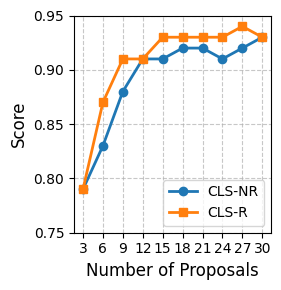
\includegraphics{imgs/prop-num-abl.png}
    \caption{Proposal Number Ablation}
\end{figure}

As shown in \ref{fig:ablation_candidates}, the performance of both CLS-NR and CLS-R improves significantly when increasing proposals from 3 to 15 (CLS-NR: $0.81 \rightarrow 0.92$, CLS-R: $0.79 \rightarrow 0.93$), but plateaus beyond 15 proposals, showing only minimal gains up to 30. Therefore, 15 proposals were used in the main experiments.

\subsubsection{Regularization Hyperparameters}
\label{sec:regularization_hyperparameters}

We conducted an ablation study to examine the impact of regularization hyperparameters $\alpha$ and $\beta$ on learning performance.
\begin{wraptable}{l}{0.6\linewidth}
    % \vspace{-0.3cm}
    \centering
    \begin{threeparttable}
        \caption{Regularization Ablation}\label{tab:ablation-on-regularization}
        \centering
        \scriptsize
        \begin{tabular}{@{}ccc|ccc@{}}\toprule
            $\alpha$  & Conv & Triv & $\beta$   & Conv & Triv \\\midrule
            $10^{-4}$ & 99   & 0    & $10^{-2}$ & 131  & 0    \\
            $10^{-5}$ & 37   & 0    & $10^{-3}$ & 37   & 0    \\
            $10^{-6}$ & 24   & 0.4  & $10^{-4}$ & 27   & 0.5  \\
            $10^{-7}$ & 13   & 0.9  & $10^{-5}$ & 12   & 1    \\
            % \hline
            0         & 11   & 1    & 0         & 11   & 1    \\
            \bottomrule
        \end{tabular}
    \end{threeparttable}
    % \vspace{-0.3cm}
\end{wraptable}
``Conv'' means the rate of convergence measured by the number of epochs before the validation loss stops decreasing for 10 epochs. ``Triv'' is the ratio of learned rules that are trivial (e.g., $\top \rightarrow \top$) across 10 runs in the ``Following'' scenario.
While varying $\alpha$ ($\beta$), the value of $\beta$ ($\alpha$) is fixed to $10^{-3}$ ($10^{-5}$).
When $\alpha = 0$ or $\beta = 0$ (i.e. no regularization), the model converges quickly (11 epochs) but learns only trivial rules.
Larger $\alpha$ ($10^{-7}$ to $10^{-4}$) and $\beta$ ($10^{-5}$ to $10^{-2}$) values increase convergence time but reduce trivial rules. We found $\alpha = 10^{-5}$ and $\beta = 10^{-3}$ an optimal choice, achieving convergence in 37 epochs with no trivial rules, balancing training efficiency and rule quality.

